\section{Himmelblau's Function}
\label{sec:app:test:himmelblau}
  The \emph{Himmelblau's function}, attributed to David Mautner 
  Himmelblau,\footnote{%
    Himmelblau, D. (1972). \enquote{Applied Nonlinear Programming}. McGraw-Hill. 
    ISBN 0-07-028921-2.
  } is a significant benchmark function in the realm of optimization, renowned
  for its complex multi-modal nature.
  Himmelblau, an American engineer, made substantial contributions to systems
  engineering and optimization theory.

  \begin{definition}[Himmelblau's Function]
    \label{def:app:test:himmelblau}
    The \emph{Himmelblau's function}, symbolized as \(f: \mathbb{R}^2 \rightarrow 
    \mathbb{R}\), is formally described as:

    \begin{equation}
      \label{eq:app:test:himmelblau}
      f(x,\, y) = (x^2 + y - 11)^2 + (x + y^2 - 7)^2
    \end{equation}
    
    Here, \(x,\, y \in \mathbb{R}\) are the decision variables, with the domains 
    \(\{x\: |\: -10 \leq x \leq 10\}\) and \(\{y\: |\: -10 \leq y \leq 10\}\).
  \end{definition}

  Distinguished by its four minima, located at \((3,\, 2)\), \((-2.805118,\, 
  3.131312)\), \((-3.779310,\, -3.283186)\), and \((3.584428,\, -1.848126)\), 
  all roughly equating to zero, this function showcases its complexity.

  Figure \ref{fig:app:test:himmelblau} portrays the multi-modal landscape of 
  Himmelblau's function through contour and surface plots, underlining its 
  inherent intricacy, and as such, its utility in the evaluation of optimization
  techniques.

  \begin{figure}[ht!]
    \centering
    \begin{subfigure}[b]{0.45\textwidth}
      \centering
      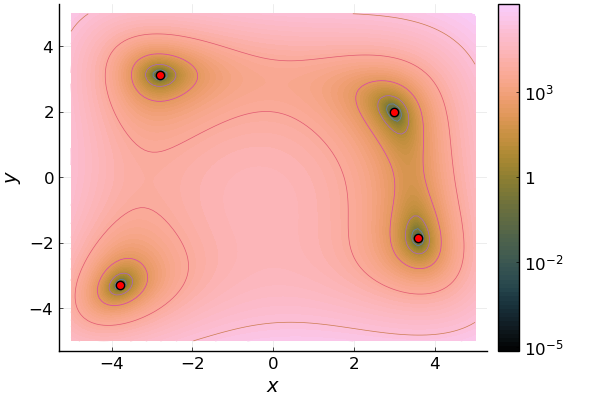
\includegraphics[width=\textwidth]
        {img/test_functions/himmelblau_contour.png}
      \caption{
        Contour plot of Himmelblau's function, the minima are signified by the 
        red dots
      }
      \label{fig:app:test:himmelblau:contour}
    \end{subfigure}
    \hfill
    \begin{subfigure}[b]{0.45\textwidth}
      \centering
      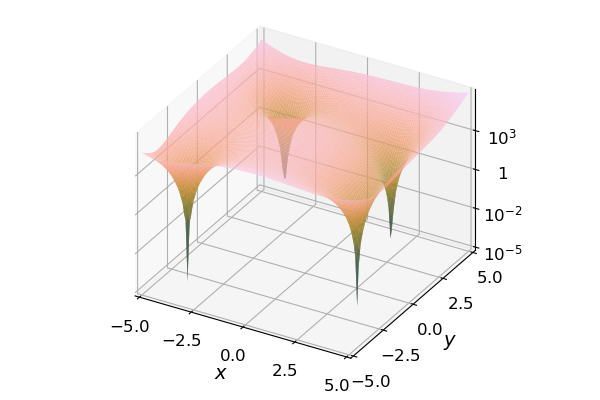
\includegraphics[width=\textwidth]
        {img/test_functions/himmelblau_surface.png}
      \caption{Surface plot of Himmelblau's function}
      \label{fig:app:test:himmelblau:surface}
    \end{subfigure}
    \caption{
      The detailed multi-modal structure of Himmelblau's function illustrated 
      through contour and surface plots
    }
    \label{fig:app:test:himmelblau}
  \end{figure}
